\documentclass[10pt, compress]{beamer}
\usetheme[conference=TCV-Topic21 Interim,venue=Lausanne, date=13/10/2017, titleprogressbar, logo=RFX-logo]{Eurof}
\usepackage{listings,amsmath,multimedia, amssymb}
\usepackage{../beamerclass/tangocolors}
\usepackage{../beamerclass/rfxcolor}
% for drawing
\usepackage{pgf}
\usepackage{tikz}
\usetikzlibrary{arrows,shapes,backgrounds}
\usepackage{../beamerclass/onimage}
\usepackage[export]{adjustbox}
\usepackage{bm}
% for font
\usepackage[absolute,overlay]{textpos}
  \setlength{\TPHorizModule}{1mm}
  \setlength{\TPVertModule}{1mm}

\usepackage[style=nature,citestyle=authoryear-comp,defernumbers=true,maxnames=2,firstinits=true,
uniquename=init,backend=bibtex8,arxiv=abs,mcite]{biblatex}
\bibliography{biblio}
\renewcommand*{\bibfont}{\footnotesize}
\renewcommand*{\citesetup}{\footnotesize}
\usepackage[export]{adjustbox}
\makeatother
\mode<presentation>
\makeatletter
% add a macro that saves its argument
\newcommand{\footlineextra}[1]{\gdef\insertfootlineextra{#1}}
\newbox\footlineextrabox
% for reducing font on a single slide
\newcommand\Fontvi{\fontsize{8}{7.2}\selectfont}
\title{Topic 21 experiment}
\date{13 Octobe 2017}
\author[Topic 21 ST]{N . Vianello and V. Naulin for the
  Topic 21 SC team}
\begin{document}
\tikzstyle{every picture}+=[remember picture]
\maketitle
\begin{frame}{TCV experiments: boundary condition}
\vspace{-1cm}
\Fontvi
\begin{itemize}
\item 2017 \textbf{objectives} listed after the General Planning Meeting
  \begin{enumerate}
  \item Provide cross-machine \alert{L-Mode} shoulder dependence on
    current both at constant Bt and at constant q$_{95}$
  \item Establish robust scenario for density shoulder profile in
        H-mode and establish dependence on fuelling/neutral
        profiles/divertor condition
  \item Study the role of ELM regimes, neutral compression, and
    particle density in filamentary transport and related shoulder
    formation.
  \item Identify the contribution of collisionality and
    seeding on filamentary transport and related shoulder
    formation.
  \item Determine the effect of filaments and shoulder
    formation on target heat loads in different Hmode plasmas.
  \end{enumerate}
\item We still have a \# 18 Shots available between Week 43 and 44
\end{itemize}
\end{frame}

\begin{frame}{Accomplished program with respect to foreseen one}
  \Fontvi
\begin{enumerate}
\item \textcolor{green}{Shape from 57088, I$_p$ = 245 kA,  Reverse B$_t$,
    density ramp from Line Average Density = 3.8e19 @ 0.5 s to 11e19 @ 1.6s,  Bt = 1.4T. Plunge @ 0.65, 1.52}
\item  \textcolor{green}{Repeat \# 1 with I$_p$=330 kA Bt=1.4T, same density ramp, same timing for plunges}
\item  \textcolor{green}{Repeat \# 1 with I$_p$=180 kA, Bt=1.4T, same density ramp, same timing for plunges}
\item  \textcolor{green}{Repeat \# 1 with q95=2.44 as \# 2, adjust Bt consequently (Bt = 1.02T)}
\item  \textcolor{green}{Repeat \# 3 with q95=2.44 as \# 2, adjust Bt consequently (Bt=0.8T)}
\item  \textcolor{red}{Shape and current from \# 1. Stop puffing once the divertor is
  formed to get low collisionality case. ECRH ramp from 0.9s (150
  kW--500 kW)}
\item  \textcolor{red}{Repeat \# 6 with intermediate density value between \# 6 and
  \#1 density at 0.65s.} 
\item  \textcolor{red}{Repeat density ramp of Shot \# 2 in DN configuration} 
\item  \textcolor{red}{Repeat density ramp of Shot \# 3 in DN configuration} 
\item \textcolor{red}{Repeat \# 1 in forward field}
\item \textcolor{red}{Repeat \# 3 in forward field}
\end{enumerate}

\end{frame}



\begin{frame}{Current scan at constant B$_{\phi}$}
\Fontvi
  \begin{columns}[c]
    \begin{column}{0.6\textwidth}
      \includegraphics<1>[width=7.cm]{../../Experiments/TCV/analysis/pdfbox/CurrentScanConstantBt}
      \includegraphics<2>[height=0.8\textheight]{../../Experiments/TCV/analysis/pdfbox/IpConstantBt_samedensity}
      \includegraphics<3>[height=0.8\textheight]{../../Experiments/AUG/analysis/pdfbox/IpConstantBt_Profiles_UsDiv}
      \includegraphics<4>[width=6.cm]{../../Experiments/TCV/analysis/pdfbox/LambdaSizeIpScanConstantBt}
    \end{column}
    \begin{column}{0.4\textwidth}
      \begin{itemize}
        \item Confirming results from Topic-25 increasing the current
          reduces the ion flux rollover density threshold
        \item Neutral compression seems slightly reduced at higher current
        \item Ohmic power different but power radiated from the LFS
          divertor seems similar among the shots
        \item Comparable H$_{\alpha}$ emission from target
        \item<2-> Profiles from RCP suggests that at lower I$_p$
          flattening is easier even with similar values of $\Lambda_{div}$
        \item<3-> Confirmed by similar observation in AUG
        \item<4> No clear evidences in terms of blob-size actually but
          analysis is limited to a single spatial region (5-10 mm from
          the separatrix) 
        \end{itemize}
    \end{column}
  \end{columns}
\end{frame}

\begin{frame}{Current scan at constant q$_{95}$}
\Fontvi
  \begin{columns}[c]
    \begin{column}{0.6\textwidth}
      \includegraphics<1>[width=7.cm]{../../Experiments/TCV/analysis/pdfbox/CurrentScanConstantQ95}
      \includegraphics<2>[height=0.8\textheight]{../../Experiments/TCV/analysis/pdfbox/IpConstantq95_samedensity}
      \includegraphics<3>[height=0.8\textheight]{../../Experiments/AUG/analysis/pdfbox/IpConstantQ95_Profiles_UsDiv}
      \includegraphics<4>[width=7.cm]{../../Experiments/TCV/analysis/pdfbox/LambdaSizeIpScanConstantQ95}
    \end{column}
    \begin{column}{0.4\textwidth}
      \begin{itemize}
        \item Unusual scenarios with B$_{phi}$ up to 0.8T. \alert{No rollover
          on at any of the current}
        \item Expected higher target neutral pressure increase at
          higher current
        \item<2-> Profiles from RCP does not exhibit a clear trend
          with the current. \alert{We should increase the number of
            points in reciproation. We lack at high density at low
            current or eventually a point at even higher current}
        \item<3|only@3> In AUG the things are different and even with the
          same q$_{95}$ flattening is easier at lower current
        \item<4> No clear evidences in terms of blob-size actually but
          analysis is limited to a single spatial region (5-10 mm from
          the separatrix)
        \end{itemize}
    \end{column}
  \end{columns}
\end{frame}
\begin{frame}{Attempt for low collisionality}
  \begin{columns}[c]
    \begin{column}{0.7\textwidth}
      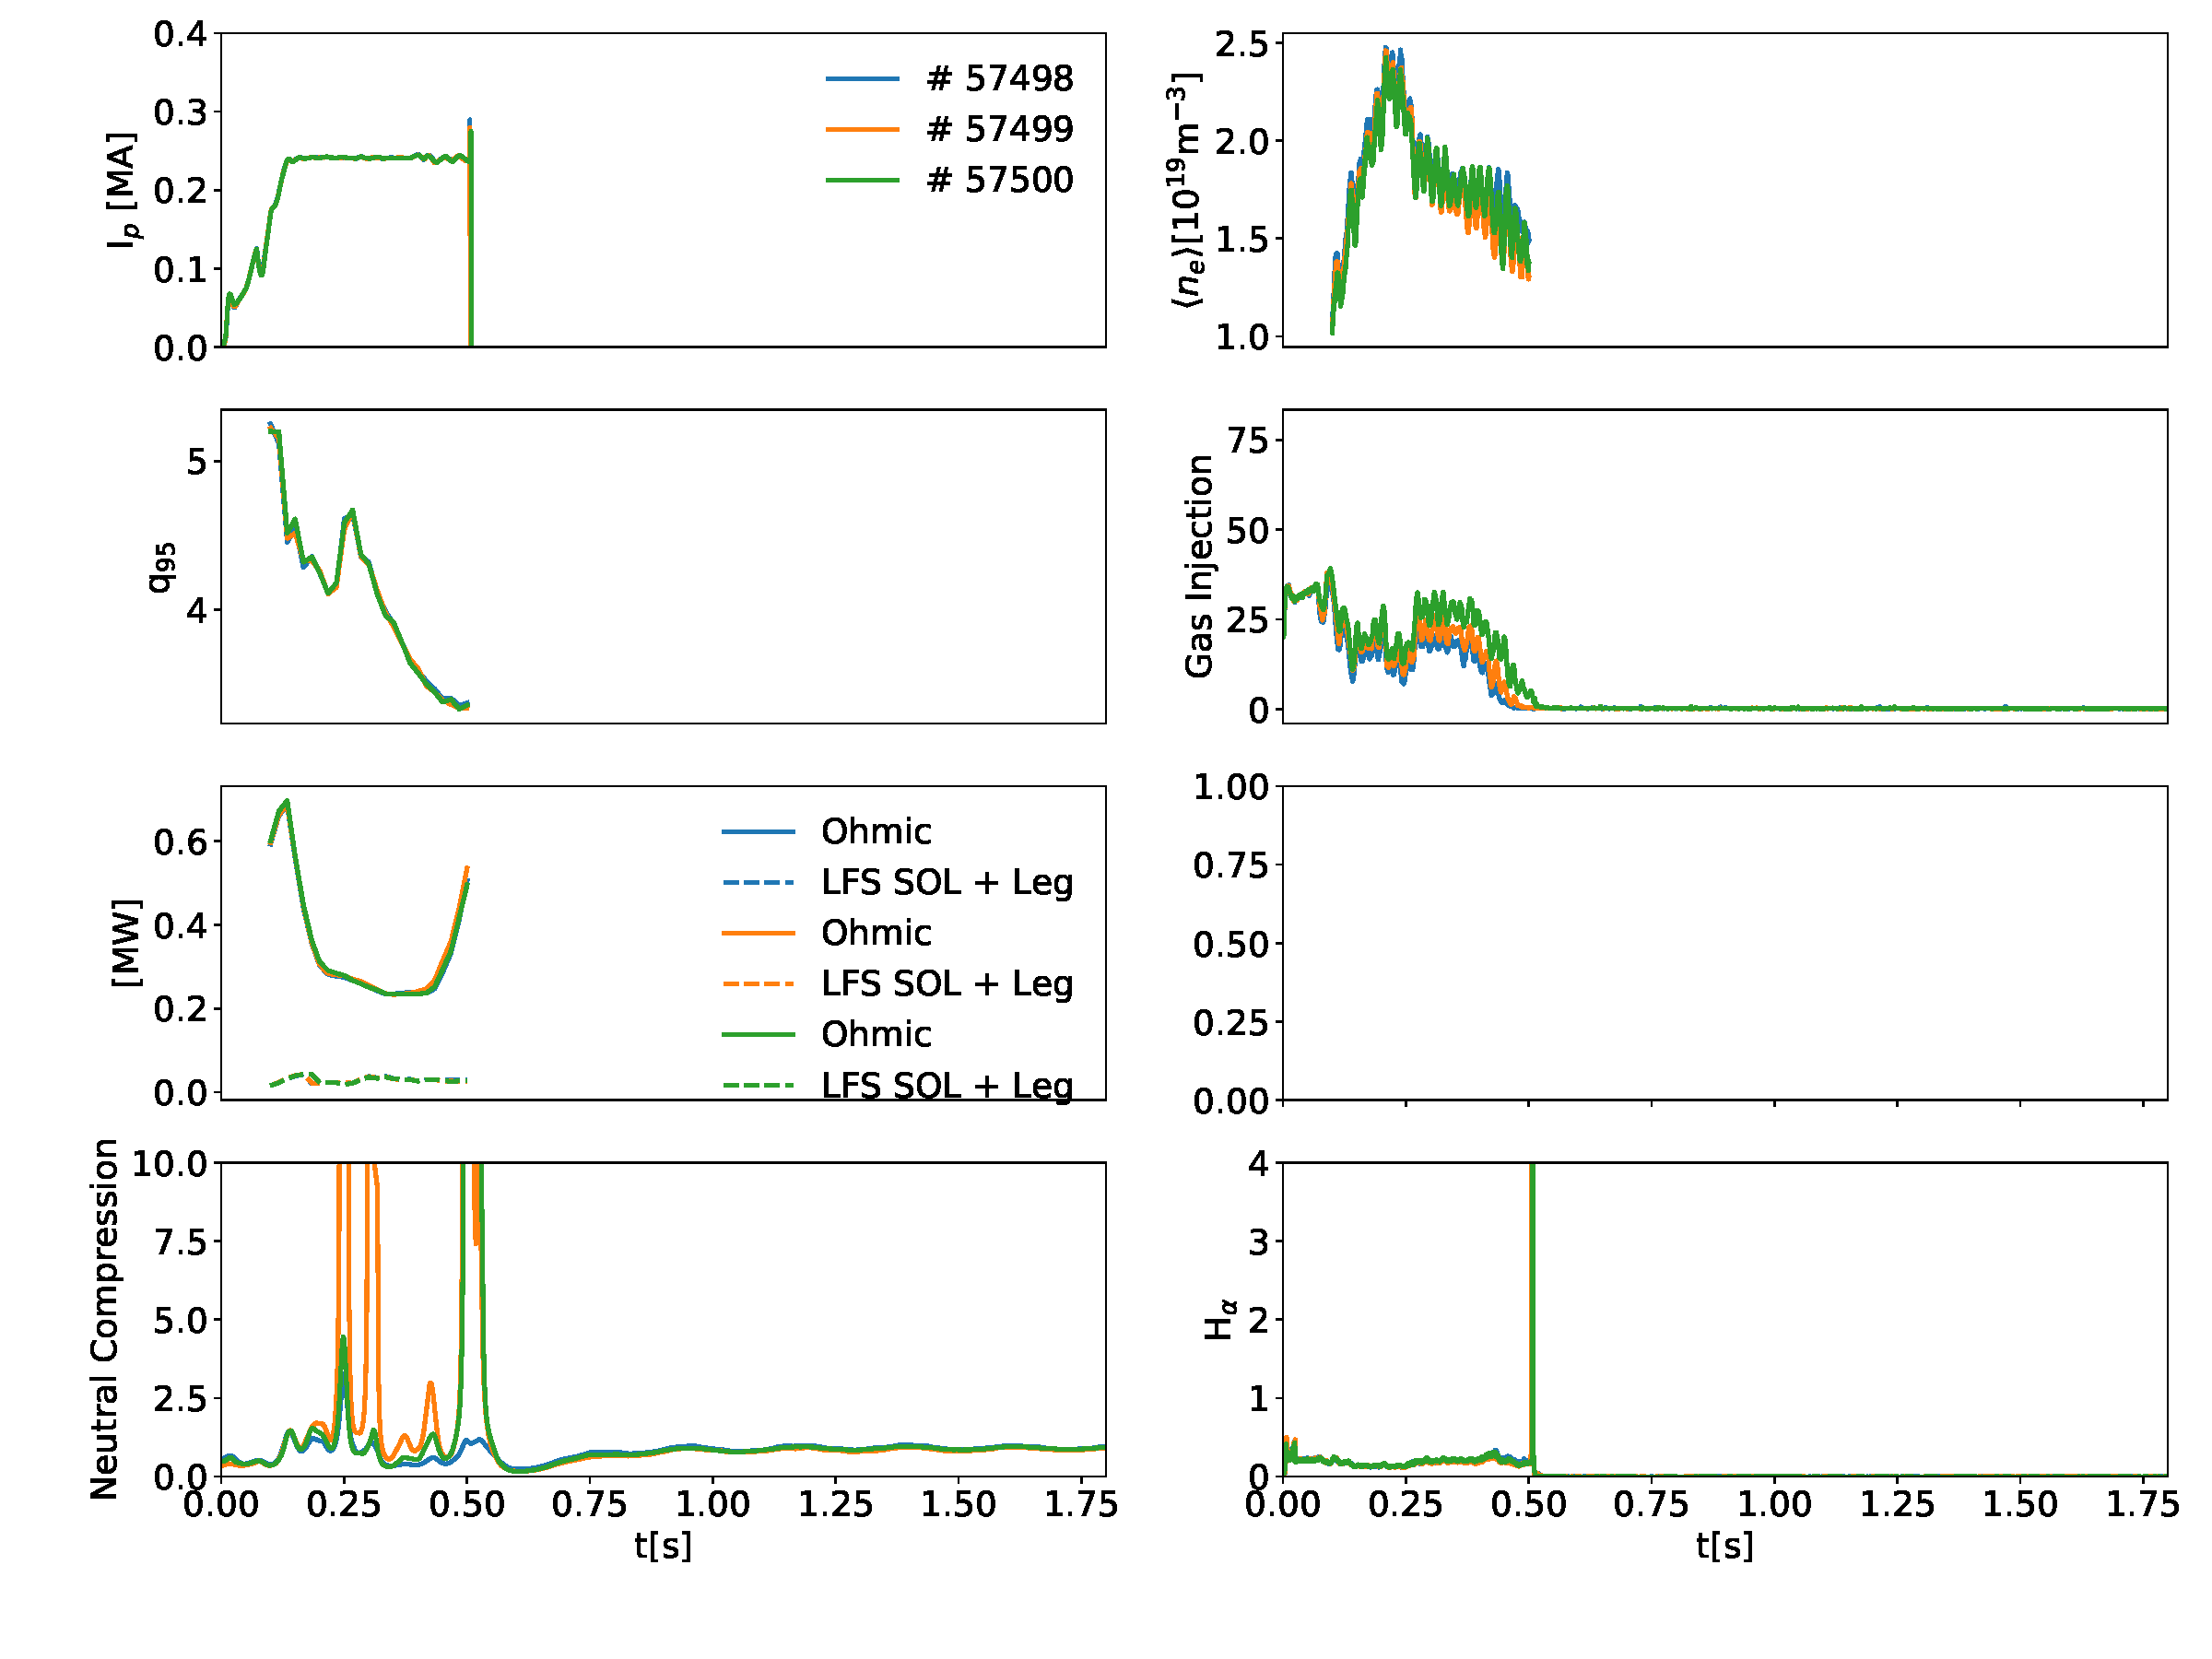
\includegraphics[width=8.cm]{../../Experiments/TCV/analysis/pdfbox/LowCollisionalityAttempt}
    \end{column}
    \begin{column}{0.3\textwidth}
      All the attempt to perform a low collisionality case disrupted
      whenever density decreases below a certain threshold
    \end{column}
  \end{columns}
\end{frame}

\begin{frame}{To be done}
  \Fontvi
  \begin{enumerate}
    \item \textcolor{orange}{ Evaluation of parallel flow profile (in
    progress)}
  \item \textcolor{orange}{ Further statistical analysis on RCP}
  \item \textcolor{red}{We could repeat a couple of shots with wall
      mounted probe in J$_{sat}$ for statistics at the wall to be
      compared with AUG}
  \item \textcolor{red}{DSS and multicam analysis}
  \end{enumerate}  
\end{frame}

\begin{frame}{To be done in L-Mode}
  \Fontvi
  \begin{enumerate}
\item  Low collisionality case useful for baseline scenario with no
  shoulder at all
\item  A point at higher current at constant B$_{\phi}$ (I don't think
  we have still room for reducing the field further)
\item  Repeat density ramp of Shot \# 2 in DN configuration at fixed B$_{\phi}$
\item  Repeat density ramp of Shot \# 3 in DN configuration at fixed B$_{\phi}$
\item  2 Shots for performing a current scan in forward B field
\end{enumerate}
\end{frame}

\begin{frame}{To be done in H-Mode}
  \Fontvi
  \begin{columns}[c]
    \begin{column}{0.5\textwidth}
      \includegraphics<1>[width=\textwidth]{../../Experiments/AUG/analysis/pdfbox/CompareShot34276_34277}
    \only<2->{
      \begin{tikzonimage}[width=\textwidth]{../../Experiments/AUG/analysis/pdfbox/EvolutionEdgeProfiles_34276_34277}
        \draw [->, ultra thick, white] (0.2, 0.45) -- (0.3, 0.55);
        \draw [->, ultra thick, white] (0.62, 0.45) -- (0.72, 0.55);
      \end{tikzonimage}   
    }
    \end{column}
    \begin{column}{0.5\textwidth}
      \begin{itemize}
        \item This is the scenario obtained in AUG without cryo-pump
          which is the best comparison possible with TCV. Density ramp
          together with N seeding for divertor cooling up to the
          degraded H-Mode
          \item<2-> This clearly exhibits a saturation of SOL profile
            which is our target
          \item<3> We will hear from Benoit and Christian which are
            the reliable scenarios which can actually been obtained so
            far on TCV
        \end{itemize}
    \end{column}
  \end{columns}
\end{frame}
\end{document}

